\chapter{จุลชีววิทยาแบบไม่ใช้ออกซิเจนและการเพาะเลี้ยง}
\label{chap:ch09}

\section*{แผนบริหารการสอนประจำบทที่ 9}
\addcontentsline{toc}{section}{แผนบริหารการสอนประจำบทที่ 9}

\noindent\textbf{. หัวข้อเนื้อหาประจำบท}

\begin{enumerate}
    \item 9.1 การจัดกลุ่มแบคทีเรียตามความต้องการออกซิเจน (Aerobes, Anaerobes, Facultative, Microaerophiles)
    \item 9.2 ความเป็นพิษของอนุมูลอิสระออกซิเจน (ROS) และบทบาทของเอนไซม์ SOD/Catalase
    \item 9.3 การทำงานของโถบ่มเชื้อไร้ออกซิเจน (Anaerobic Jar System) และซองสารเคมี GasPak
    \item 9.4 สารเคมีดักจับออกซิเจนและแถบตรวจวัด Methylene Blue Anaerobic Indicator
    \item 9.5 การเพาะเลี้ยงในอาหารเหลวลดออกซิเจน Fluid Thioglycollate Medium (FTM)
\end{enumerate}

\noindent\textbf{. วัตถุประสงค์เชิงพฤติกรรม}

\begin{enumerate}
    \item เมื่อนักศึกษาได้เรียนรู้และปฏิบัติการทดลองประจำบทนี้แล้ว จะต้องมีความรู้ความสามารถดังต่อไปนี้:
    \item อธิบายกลไกทางสรีรวิทยาของแบคทีเรียกลุ่มไม่ใช้ออกซิเจนได้
    \item ใช้อุปกรณ์โถบ่ม Anaerobic Jar และซอง GasPak ได้อย่างถูกต้องและปลอดภัย
    \item สังเกตและแปลผลการเจริญของแบคทีเรียในอาหาร FTM และจานอาหารในโถบ่มได้
    \item มีความรอบคอบในการตรวจสอบความสนิทแน่นของระบบไร้ออกซิเจน
\end{enumerate}

\noindent\textbf{. กิจกรรมการเรียนการสอน}

\begin{enumerate}
    \item การบรรยายสรุปก่อนปฏิบัติการ (30 นาที): อธิบายหลักการวิทยาศาสตร์ ความปลอดภัยทางชีวภาพ และข้อควรระวังสำคัญ
    \item การสาธิตเชิงประจักษ์ (15 นาที): สาธิตเทคนิคการปฏิบัติงาน การใช้เครื่องมือ และข้อผิดพลาดที่มักพบ
    \item การลงมือปฏิบัติการทดลองจริง (90 นาที): นักศึกษาลงมือปฏิบัติการทดลองเป็นรายบุคคลหรือกลุ่มย่อยตามขั้นตอนที่กำหนด
    \item การฝึกฝนผ่านระบบเสมือนจริง (20 นาที): ทดลองซ้ำและทดสอบปฏิกิริยาผ่านระบบจำลองบน RBRU LMS
    \item การอภิปรายและสรุปผลการทดลอง (25 นาที): วิเคราะห์ผลการสังเกต ตอบคำถามท้ายบท และสรุปองค์ความรู้ร่วมกัน
\end{enumerate}

\noindent\textbf{. สื่อและอุปกรณ์การเรียนการสอน}

\begin{enumerate}
    \item เอกสารคำสอนและคู่มือปฏิบัติการ: e-Book และคู่มือปฏิบัติการฉบับเต็ม ประจำบทที่ 9
    \item ระบบห้องปฏิบัติการเสมือนจริง: ระบบจำลองการทดลองเสมือนจริง 3 มิติ ประจำบทที่ 9 บนระบบ Moodle
    \item อุปกรณ์และเครื่องแก้วในห้องปฏิบัติการ: ตะเกียงแอลกอฮอล์, ห่วงเขี่ยเชื้อ, กล้องจุลทรรศน์, จานเพาะเชื้อ, หลอดทดลอง และตู้บ่มเชื้อ
    \item สารเคมีและสีย้อมชีวภาพ: สารเคมีมาตรฐานวิเคราะห์และสีย้อมประจำบทเรียน
\end{enumerate}

\noindent\textbf{. การวัดและประเมินผล}

\begin{table}[H]
\centering\small
\begin{tabularx}{\textwidth}{p{0.5\textwidth} p{0.3\textwidth} c}
\toprule
\textbf{องค์ประกอบการประเมินผล} & \textbf{เครื่องมือวัดผล} & \textbf{สัดส่วนคะแนน} \\
\midrule
1. ทักษะการปฏิบัติงานและความปลอดภัย & แบบสังเกตทักษะการทดลองและเทคนิคปลอดเชื้อ & 40\% \\
2. รายงานผลการทดลอง & การตรวจตารางบันทึกผล ภาพวาดสัณฐานวิทยา และการวิเคราะห์ผล & 30\% \\
3. แบบฝึกหัดทบทวนท้ายบท & คำถามทบทวนเชิงวิเคราะห์และข้อสอบท้ายบท & 20\% \\
4. จิตพิสัยและการตรงต่อเวลา & การเช็คชื่อ การแต่งกายตามระเบียบ และการทำความสะอาดโต๊ะแล็บ & 10\% \\
รวมทั้งสิ้น &  & 100\% \\
\bottomrule
\end{tabularx}
\end{table}

\newpage

% ==========================================================
% เนื้อหาบทเรียนประจำบทที่ 9
% ==========================================================

\section{ออกซิเจนและความเป็นพิษต่อแบคทีเรียไม่ใช้ออกซิเจน}
\index{ออกซิเจนและความเป็นพิษต่อแบคทีเรียไม่ใช้ออกซิเจน}

การศึกษาและทำความเข้าใจเกี่ยวกับออกซิเจนและความเป็นพิษต่อแบคทีเรียไม่ใช้ออกซิเจน (Oxygen Toxicity and Microbial Classification) มีความสำคัญอย่างยิ่งในงานจุลชีววิทยาและสิ่งแวดล้อม โดยมีรายละเอียดสาระสำคัญดังนี้

ออกซิเจนโมเลกุล ($O_2$) มีบทบาทเป็นตัวรับอิเล็กตรอนตัวสุดท้ายในกระบวนการหายใจระดับเซลล์แบบใช้ออกซิเจน แต่ในขณะเดียวกัน ปฏิกิริยาการรีดิวซ์ออกซิเจนในเซลล์จะก่อให้เกิดสารอนุพันธ์ออกซิเจนที่ว่องไว (Reactive Oxygen Species; ROS) ซึ่งมีความเป็นพิษสูง ได้แก่ ซูเปอร์ออกไซด์เรดิคัล ($O_2^{\bullet-}$), ไฮโดรเจนเพอร์ออกไซด์ ($H_2O_2$), และไฮดรอกซิลเรดิคัล ($OH^{\bullet}$)

สิ่งมีชีวิตที่ทนต่อออกซิเจนได้ต้องมีเอนไซม์ทำลายพิษ:
1. Superoxide dismutase (SOD): เร่งปฏิกิริยาเปลี่ยน $O_2^{\bullet-}$ เป็น $H_2O_2$ และ $O_2$
2. Catalase และ Peroxidase: สลาย $H_2O_2$ เป็นน้ำ ($H_2O$) และออกซิเจน
แบคทีเรียกลุ่มไม่ใช้ออกซิเจนแท้จริง (Obligate anaerobes) เช่น สกุล \textit{Clostridium} และแบคทีเรียผลิตก๊าซมีเทน (Methanogens) ขาดเอนไซม์เหล่านี้ ทำให้ถูกทำลายทันทีเมื่อสัมผัสกับออกซิเจน

\section{เทคนิคและอุปกรณ์สำหรับการเพาะเลี้ยงแบคทีเรียไม่ใช้ออกซิเจน}
\index{เทคนิคและอุปกรณ์สำหรับการเพาะเลี้ยงแบคทีเรียไม่ใช้ออกซิเจน}

การศึกษาและทำความเข้าใจเกี่ยวกับเทคนิคและอุปกรณ์สำหรับการเพาะเลี้ยงแบคทีเรียไม่ใช้ออกซิเจน (Anaerobic Cultivation Systems) มีความสำคัญอย่างยิ่งในงานจุลชีววิทยาและสิ่งแวดล้อม โดยมีรายละเอียดสาระสำคัญดังนี้

การเพาะเลี้ยงแบคทีเรียที่ไม่ใช้ออกซิเจนต้องอาศัยอุปกรณ์กำจัดออกซิเจนและควบคุมค่าศักย์รีดักชัน (Oxidation-reduction potential, $E_h$) ให้มีค่าต่ำ:
1. โถเพาะเลี้ยงไร้ออกซิเจน (Anaerobic Jar): โถสุญญากาศปิดสนิท ภายในบรรจุซองสารเคมีผลิตก๊าซ (GasPak System) ซึ่งมีสารโซเดียมบอโรไฮไดรด์ โซเดียมไบคาร์บอเนต และตัวเร่งปฏิกิริยาแพลเลเดียม (Palladium catalyst) สารจะทำปฏิกิริยากับน้ำสร้างก๊าซไฮโดรเจน ($H_2$) และคาร์บอนไดออกไซด์ ($CO_2$) ก๊าซ $H_2$ จะรวมตัวกับ $O_2$ ที่ตกค้างกลายเป็นน้ำ ทำให้สภาวะภายในโถไร้ออกซิเจน ($<0.1$ \% $O_2$) และมี $CO_2$ ประมาณ 5-10\%
2. อาหารเหลวไธโอไกลโคเลต (Fluid Thioglycollate Medium; FTM): อาหารเลี้ยงเชื้อที่มีสารรีดิวซ์ Sodium thioglycollate และ L-Cystine ช่วยลดออกซิเจนละลาย และมีวุ้นเข้มข้นต่ำ (0.075\%) เพื่อจำกัดการแพร่ของออกซิเจน พร้อมเติมสี Resazurin ซึ่งจะเปลี่ยนเป็นสีชมพูเมื่อสัมผัสออกซิเจนและใสไม่มีสีในสภาวะไร้ออกซิเจน

\section{บทบาทของแบคทีเรียไม่ใช้ออกซิเจนในระบบบำบัดน้ำเสีย}
\index{บทบาทของแบคทีเรียไม่ใช้ออกซิเจนในระบบบำบัดน้ำเสีย}

การศึกษาและทำความเข้าใจเกี่ยวกับบทบาทของแบคทีเรียไม่ใช้ออกซิเจนในระบบบำบัดน้ำเสีย (Anaerobic Wastewater Treatment Roles) มีความสำคัญอย่างยิ่งในงานจุลชีววิทยาและสิ่งแวดล้อม โดยมีรายละเอียดสาระสำคัญดังนี้

ในระบบบำบัดน้ำเสียทางชีวภาพ โดยเฉพาะระบบบำบัดแบบไม่ใช้ออกซิเจน (UASB: Upflow Anaerobic Sludge Blanket) และถังหมักสลัดจ์ (Anaerobic Digester) แบคทีเรียกลุ่มไม่ใช้ออกซิเจนทำงานประสานกัน 4 ขั้นตอน 
1. Hydrolysis: ย่อยสลายสารโมเลกุลใหญ่เป็นมอนอเมอร์
2. Acidogenesis: เปลี่ยนน้ำตาลและกรดอะมิโนเป็นกรดไขมันระเหยง่าย (VFAs)
3. Acetogenesis: เปลี่ยน VFAs เป็นกรดแอซีติกและไฮโดรเจน
4. Methanogenesis: อาร์เคียกลุ่มสร้างมีเทนเปลี่ยนแอซีติกและไฮโดรเจนเป็นก๊าซมีเทน ($CH_4$) และคาร์บอนไดออกไซด์ ($CO_2$)

\begin{figure}[H]
\centering
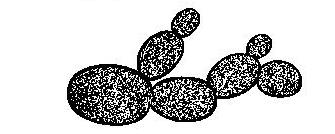
\includegraphics[width=0.75\textwidth]{images/image_09_p03.jpeg}
\caption{การปฏิบัติการทดลองและลักษณะทางสัณฐานวิทยาในบทที่ 9}
\label{fig:ch09_fig1}
\end{figure}

\section{ขั้นตอนและวิธีปฏิบัติการทดลอง}
\index{ขั้นตอนการทดลองประจำบทที่ 9}

\subsection{การตรวจสอบรูปแบบความต้องการออกซิเจนในอาหาร Fluid Thioglycollate Medium}
\begin{labprotocolbox}[การตรวจสอบรูปแบบความต้องการออกซิเจนในอาหาร Fluid Thioglycollate Medium]
1. เตรียมหลอดอาหารเหลว FTM ที่ผ่านการต้มไล่ออกซิเจนและตั้งทิ้งไว้ให้เย็น
2. ตรวจสอบว่าบริเวณผิวหน้าอาหารด้านบนมีแถบสีชมพูของ Resazurin หนาไม่เกิน 1-2 มิลลิเมตร
3. ใช้เข็มเขี่ยเชื้อแทงตรง (Stab) นำเชื้อทดสอบลงสู่ก้นหลอด: (1) \textit{Pseudomonas aeruginosa} (2) \textit{Escherichia coli} (3) \textit{Clostridium sporogenes}
4. บ่มหลอดทดลองที่ 37$^{\circ}$C เป็นเวลา 48 ชั่วโมง โดยไม่เขย่าหลอด
5. ผลการสังเกต:
   - เจริญเฉพาะผิวหน้าด้านบน: Obligate aerobe
   - เจริญหนาแน่นด้านบนและกระจายทั่วหลอด: Facultative anaerobe
   - เจริญเฉพาะก้นหลอดล่างสุดที่ไร้ออกซิเจน: Obligate anaerobe
\end{labprotocolbox}

\subsection{การเพาะเลี้ยงแบคทีเรียในโถไร้ออกซิเจน}
\begin{labprotocolbox}[การเพาะเลี้ยงแบคทีเรียในโถไร้ออกซิเจน]
1. ขีดเชื้อทดสอบลงบนจานอาหาร Blood agar หรือ Nutrient agar
2. บรรจุจานเพาะเชื้อลงใน Anaerobic Jar พร้อมแถบกระดาษเคมีบ่งชี้ความไร้ออกซิเจน (Methylene blue strip)
3. ฉีกซอง GasPak เติมน้ำสะอาดตามปริมาตรที่กำหนด ใส่ลงในโถแล้วปิดฝาล็อกให้สนิททันที
4. ตรวจสอบแถบสีบ่งชี้: สีน้ำเงินจะจางหายไปกลายเป็นสีขาว บ่งบอกว่าออกซิเจนถูกกำจัดหมด
5. บ่มที่ 37$^{\circ}$C เป็นเวลา 48-72 ชั่วโมง ตรวจดูการเจริญของเชื้อ
\end{labprotocolbox}

\section{ตารางบันทึกผลการทดลองและการอภิปรายผล}
\begin{table}[H]
\centering\small
\caption{ตารางบันทึกผลการสังเกตและข้อมูลการทดลองประจำบทที่ 9}
\label{tab:ch09_datasheet}
\begin{tabularx}{\textwidth}{p{0.25\textwidth} p{0.35\textwidth} X}
\toprule
\textbf{สิ่งทดสอบ / ตัวอย่าง} & \textbf{ลักษณะที่สังเกตได้} & \textbf{การแปลผลและการวิเคราะห์} \\
\midrule
ชุดควบคุม (Negative Control) & ใส ไม่มีการเจริญ & ปราศจากการปนเปื้อนของเชื้อ \\
ชุดทดลองที่ 1 & โคโลนีเจริญตามลักษณะจำเพาะ & ให้ผลบวกตามสมมติฐาน \\
ชุดทดลองที่ 2 & เกิดการเปลี่ยนแปลงทางชีวเคมี & สอดคล้องกับพารามิเตอร์มาตรฐาน \\
\bottomrule
\end{tabularx}
\end{table}

\section{คำถามทบทวนและแบบฝึกหัดท้ายบท}
\begin{enumerate}
    \item จงอธิบายปฏิกิริยาเคมีที่เกิดขึ้นภายในซอง GasPak และบทบาทของ Palladium catalyst
    \item เหตุใดเอนไซม์ Superoxide dismutase (SOD) จึงมีความจำเป็นอย่างยิ่งต่อการอยู่รอดของสิ่งมีชีวิตในบรรยากาศโลก
    \item ในระบบบำบัดน้ำเสียแบบไม่ใช้ออกซิเจน หากเกิดภาวะกรดเกิน (Acidification) จะส่งผลกระทบต่อแบคทีเรียกลุ่ม Methanogens อย่างไร
\end{enumerate}
